 
\documentclass[10pt, conference, compsocconf]{IEEEtran}


% *** CITATION PACKAGES ***
\usepackage{amsmath}
\usepackage{fullpage}
\usepackage[utf8]{inputenc}
\usepackage{mathtools}
\usepackage{amssymb}
\usepackage{graphicx}
\usepackage{caption}
\usepackage{subcaption}
\usepackage{amsthm}
\usepackage{aliascnt}

\DeclarePairedDelimiter{\ceil}{\lceil}{\rceil}

\usepackage[usenames,dvipsnames]{color}
\usepackage[colorlinks=true,urlcolor=OliveGreen,citecolor=Blue]{hyperref}

\usepackage{soul}
\usepackage{xspace}

 

\newtheorem{theorem}{Theorem}
\newtheorem{corollary}{Corollary}[theorem]
\newtheorem{lemma}[theorem]{Lemma}

\newcommand{\todo}[1]{{\color{red}\textbf{\hl{#1}}\xspace}}

%\graphicspath{{C:\Users\Manmohan\Documents\GitHub\research}}

% *** GRAPHICS RELATED PACKAGES ***
% 
\ifCLASSINFOpdf
  % \usepackage[pdftex]{graphicx}
  % declare the path(s) where your graphic files are
  % \graphicspath{{../pdf/}{../jpeg/}}
  % and their extensions so you won't have to specify these with
  % every instance of \includegraphics
  % \DeclareGraphicsExtensions{.pdf,.jpeg,.png}
\else
 
\fi

% correct bad hyphenation here
\hyphenation{op-tical net-works semi-conduc-tor}


\makeatletter
\renewcommand*{\thetable}{\arabic{table}}
\renewcommand*{\thefigure}{\arabic{figure}}
\let\c@algocf\@undefined
\newaliascnt{algocf}{figure}
\let\c@table\@undefined
\newaliascnt{table}{figure}
\let\c@table\c@figure

\makeatother

\begin{document}

\title{Replicated Data Placement for Uncertain Scheduling}


\author{\IEEEauthorblockN{Manmohan Chaubey, Erik Saule }
\IEEEauthorblockA{Department of Computer Science\\
 University of North Carolina at Charlotte\\
 Charlotte, USA\\
 Email: mchaubey@uncc.edu, esaule@uncc.edu}
}

\maketitle


\begin{abstract}
  Scheduling theory is a common tool to analyze the
  performance of parallel and distributed computing systems, such as their load
  balance. How to distribute the input data to be able to execute a
  set of tasks in a minimum amount of time can be modeled as a
  scheduling problem. Often these models assume that the computation
  time required for each task is known accurately. However in many
  practical case, only approximate values are available at the time of
  scheduling.

  In this paper, we investigate how replicating the data required by
  the tasks can help coping with the inaccuracies of the processing
  times. In particular, we investigate the problem of scheduling
  independent tasks to optimize the makespan on a parallel system
  where the processing times of tasks are only known up to a
  multiplicative factor. The problem is decomposed in two phases: a
  first offline phase where the data of the tasks are placed and a second
  online phase where the tasks are actually scheduled.

  For this problem we investigate three different strategies, each
  allowing a different degree of replication of jobs: a) No
  Replication b) Replication everywhere and c) Replication in
  groups. We propose approximation algorithms and theoretical lower
  bound on achievable approximation ratios.  This allows us to study
  the trade-off between the number of replication and the guarantee on
  the makespan.
\end{abstract}

\begin{IEEEkeywords}
Scheduling; Uncertainty; Robustness; Replication; Approximation Algorithms; Parallel System

\end{IEEEkeywords}


\IEEEpeerreviewmaketitle

\section{Introduction}

\todo{the introduction should be structure as follow.}

\todo{one paragraph on scheduling as a tool for analyzing and
  optimizing parallel and distributed systems.Mention that in
  scheduling often processing time are known. But in practice not so
  much. Give a few references on the difficulty of predicting runtimes
  in job scheduler.}
  
  In parallel and distributed computing, tasks are processed simultaneously on different machines to minimize time to complete the processing of all the tasks.   The scheduling for the set of tasks on a given set of machines are usually determined with a goal to optimize certain parameter, such as makespan.  The Scheduling study is also used to provide insight into the performance of parallel and distributed computing systems, such as their load balance.  The problem of distributing the input data to execute a set of tasks in a minimum amount of time can be formulated as a scheduling problem.  Often these scheduling problems are modeled based on the assumption that the computation time required for each task is known accurately; while, in a more practical scenario, only approximate values for the computation times of the tasks can be determined at the time of scheduling.

\todo{we need a paragraph on data placement. essentially: uncertainty
  would not be a problem if the schedules could be dynamically
  changed. But in practice, the task has to run somewhere because its
  input data is there. For instance Hadoop, dooc+laf; but essentially
  in any parallel code. Even if some middleware support executing the
  task everywhere it pays an overhead for transferring data.}

\todo{one approach for the problem is to build robust schedule. define
  robust schedule and give few quick pointers. What is better is to be
  able to arrange the schedule at runtime. What we investigate: using
  data replication to give room to the scheduler to move tasks
  around. Can it help?}

\todo{In paragraph that gives document organization. In section foo,
  we present this. In section bar we present that. This is where
  contribution should be presented. no need to give formula.}

Many real world scheduling problems related to task allocation in
parallel machines are uncertain in nature. This fact makes the class
of problem known as 'scheduling with uncertainty' or 'robust'
scheduling an important and most studied problem in
Scheduling. Robustness is the measure of to what extent an algorithm
can cope with uncertainties in a scheduling problem. Often in
scheduling problems the exact processing time of a job is not known
initially at the time of planning for job- allocation to different
machines, but they have a range outside which their values cannot
lie. The fact gives a basis to estimate the processing times and to
take job assignment decision based on these estimated values. The
actual processing time of a job can vary drastically from its
estimated one. So, any algorithm have to incur the cost of estimation
which impacts its performance negatively. A robust approach deals with
uncertainty in input parameters to minimize this cost.


The objective of our research is to study the affect on performance of
parallel machine scheduling when jobs are scheduled based on their
estimated values of processing times, and to propose scheduling
approaches that optimizes the performance in this environment. Data
placement and replication techniques can be useful in the scenario of
uncertain processing times of tasks. Effective data placement using
replication strategy allows better load balancing and hence reduces
turnaround job time. This paper is important in the sense that it
proposes different models depending upon different scenarios and
compares them based on approximation ratio and replication they
allow. Replication strategy that allows to place data in a wisely
manner offers a faster access to files required by jobs, hence
increases the job execution's performance. Replication helps in load
balancing but it have cost attached with it as it usually increases
resource usage~\cite{DBLP:journals/corr/WangJW14}. The paper deals
with this problem and chooses the scenario in which replication is
beneficial. Thus our research focus on two area of scheduling problem
i.e. task uncertainty and replication using data placement. The
scheduling problem related to data placement and task allocation is
common in heterogeneous systems and often dealt with common
approach. This paper draws qualitative analysis of the effect of
replication in data placement for uncertain scheduling with inexact
processing time of a task.

The remaining of the paper is organized as follows: we describe system
model and notations in section~\ref{sec2}. Related works are touched
in section~\ref{sec3}.  Sections~\ref{sec4}-~\ref{sec6} describes the
3 different strategies- a)No replications, b)replication is done
everywhere and c)replication is done within a group. \todo{expand per
  section}. The respective sections describe derivation of competitive
ratios for each of these strategies. Section~\ref{sec7} summarizes the
results of 3 models based on experimental results.

\section{Problem Definition}\label{sec2}
Let $J$ be a set of $n$ jobs which need to be scheduled onto a set $M$
of $m$ machines. We will use interchangeably the terms machines and
processors. Also we will use interchangeably the terms jobs and
tasks. We are considering the problems where the scheduler does not
know the processing time $p_i$ of task $i$ exactly before the task
completes.  But the scheduler has access to some estimation of the
processing time $\tilde{p_i}$ of task $i$ before making any scheduling
decisions. We assume that the actual processing time $p_i$ of a task
$i$ is within a multiplicative factor $\alpha$ of the estimated
processing time $\tilde{p_i}$. $\alpha$ is a quantity known to the
scheduler. In other words the scheduler knows that:
 \begin{equation}\label{eq1}
\frac{\tilde{p}_{i}}{\alpha}\leq p_{i}\leq \alpha \tilde{p}_{i}
\end{equation}


Assuming that the processing time of the tasks is known to be in an
interval is reasonable in many application scenarios. One could derive
bounds experimentally using machine learning techniques: for
instance~\cite{You14-ICPP} used Support Vector Machines to predict the time it
will take to run graph traversal algorithms. Models of runtime of
algorithms can also be derived analytically:
in~\cite{Erlebacher14-ICS} the authors provide bounds for the
performance of various sparse linear algebra operations using only the
size of the matrices and vector involved.

The problem is to optimize the makespan, $C_{max}$. \todo{Define
  makespan formally. Probably better if we push that at the end of the
  section.} Makespan is the load on machine which processes the latest task. $C_{max}^{*}$ denotes optimal makespan of a schedule $S$.

\todo{Write it so that the problem is defined in two phases, what ever
  the strategy. the strategy we follow does not change the problem.}
The scheduling for the problem is defined in two phases.  Phase 1 chooses where data to be replicated using estimated processing time $\tilde p_j $, for each of the task $j$. The phase takes $\tilde{p_j}$, $m$ and $\alpha$ as input and outputs set of machines, $M_j \subseteq M $ where a task $j$ can be scheduled.

Phase 2 takes output of phase 1 as its input and maps a task $j$ to a machine within the set of machines $M_j$ to which $j$ was allocated in phase 1.  For each  machine $i$ phase 2 outputs a set of tasks $E_i \subseteq J$ assigned to the machine $i$.  The Phase chooses actual schedule with semi-clairvoyant algorithm which uses only approximate knowledge of initial processing time, and after scheduling the task the actual $p_i$ is known.  With objective to find schedule which minimizes
makespan, we investigate greedy algorithms for each of the problem
models and prove their competitive ratios. \todo{what we investigate
has nothing to do here. This is a problem definition.}


\section{Related Work}\label{sec3}

\todo{First with $\alpha=1$ this is the classical scheduling
  problem.}\todo{NP-Hardness. cite garey johnson.} We have used
Graham's List Scheduling (LS)~\cite{Graham66} and Largest Processing
Time (LPT) algorithms~\cite{Graham69boundson} to derive approximation
ratios in different scenarios. The LS algorithm takes tasks one at a
time and assign it to the processor having least load at that time. LS
is 2-approximation algorithm and is widely used in online scheduling
problems. LPT sorts tasks in decreasing order of processing time and
assign them one at a time in this order to the processor with the
smallest current load. The LPT algorithm has worst case performance
ratio as $\frac{4}{3}-\frac{1}{3m} $ in an offline setting. Depending
upon which among these two algorithms suits more for a problem model
we have used these algorithms accordingly. \todo{PTAS from hochbaum shmoys}



Based on various models of describing uncertainty in input parameter,
uncertainty problems can be approached by various methodologies
including Reactive, stochastic, fuzzy and Robust
approach~\cite{DBLP:journals/cce/LiI08}. The bounded uncertainty model
assumes that an input parameter have value between a lower and upper
bound and is usually dealt with robust approach or sensitivity
analysis\todo{cite}. We are more interested in robust approach to deal
with uncertainty. \todo{ Be factual,
  this paper takes that approach and shows that or applies it to
  that.} Wierman and Nuyens~\cite{conf/sigmetrics/WiermanN08}
introduce SMART as classification to understand size based policies
and draw analytical co-relation between response time and estimated
job size in single server problem. Dealing with uncertainty problems
with robust approach is widely used in practicality in the area of
MapReduce~\cite{Kavulya:2010:ATP:1844765.1845224}~\cite{Verma:2011:AAR:1998582.1998637},
Hadoop~\cite{Wolf:2010:FSA:2023718.2023720}~\cite{White:2009:HDG:1717298},
databases~\cite{Lipton199518} and web
servers~\cite{Cardellini99dynamicload}. HSFS and FLEX schedulers are
proposed which provides robustness in scheduling against uncertain Job
Size ~\cite{Wolf:2010:FSA:2023718.2023720} \cite{6691554}. Cannon and
Jeannot ~\cite{cj09c} provides scheduling heuristics that optimizes
both makespan and robustness in scheduling task graph on heterogeneous
system. \todo{This is not the contribution of this paper. It is mostly
  trying to understand what is the correct metric for measuring the
  robustness of a schedule. }

Most of the work on robust scheduling uses scenarios in problem
formulation to structure variability of uncertain parameter. \todo{What does a scenario means in this context.} Daniels and Kouvelis~\cite{citeulike:8334169} used scenarios to formulate
branch and bound based robust scheduling to cope uncertainty in
processing time of jobs in single machine. Davenport, Gefflot, and Bek
used slack based technique to add extra time to cope with
uncertainty~\cite{Davenport_slack-basedtechniques}. Gatto and Widmayer
derives bounds on competitive ratio of Graham’s online algorithm in
scenario where processing times of jobs either increase or decrease
arbitrarily due to perturbations~\cite{Gatto07}.  Their notion of
perturbed processing times is similar to our definition of estimated
processing times which can increase or decrease to actual processing
times once the jobs are processed. But unlike our work they considered
increment and decrement of job processing times as different problem
scenario. We have approached the problem with worst case scenario
where some tasks may increase and some may decrease in the same
schedule.
  
\todo{This is related works, this is not about what we do.} We have
used pro-active approach to deal with uncertainty. Through this
research we study effect of load balancing in scenario of uncertain
processing times. Based on different task assignment criteria we
propose 3 models for our problem definition, offering different degree
of task replication for load balancing. Data placement and replication
methodologies are highly used in distributed systems including
peer-to-peer and Grid systems to achieve effective data management and
improve
performance~\cite{Cirne2007213}\cite{Abawajy}\cite{4215379}. Our
notion of using replication is to increase data availability thereby
enhancing system reliability against uncertainties. With focus on
studying replication affect on performance of a schedule under
uncertainty, we have not considered cost of replication in terms of
memory utilization. Our work considers an ideal case where storage is
sufficient.  Similar work is done by Tse~\cite{DBLP:journals/tc/Tse12}
who used selective replication of documents in bi criteria problem of
minimizing load and memory in distributed file servers.


\subsection{Our Contribution}

\todo{Why do we have contribution here?}

We study the effect of load balancing through replication in classic
problem of scheduling jobs with uncertain processing times with
objective to optimize makespan. We propose 3 models based on different
degree of of replication they allow: a)No Replication i.e. $|M_j|=1
$,b) Replication is done every where i.e.$|M_j|=|M|$ and c)
Replication in groups i.e $|M_j|= m/k$ where $k$ is number of groups
each having $m/k$ processors . For each of the models we propose a two
phase algorithm based on Graham's LS and LPT; and derive performance
ratio for each. For $|M_j|=1 $, we prove that there is no algorithm
which give better performance than $\alpha^2$. Our algorithm for the
model give $\frac{2\alpha^{2}m}{2\alpha^{2}+ m-1}$ approximation. For
models with replications $|M_j|=|M|$ and $|M_j|= m/k$ the algorithms
give performance ratio of $ 1 + (\frac{m-1}{m})\frac{\alpha^{2}}{2}$
and $\frac{k\alpha^{2}}{\alpha^{2}+k-1}\left[1+ {\frac{k-1}{m}}
\right]+ {\frac{m-k}{m}}$ respectively.

\section{Strategy 1: No Replication}\label{sec4}


This section model considers the situation where the data of each task
is restricted to be on only one machine, i.e. $\forall j, |M_j|=1$.
We have a set $J$ of $ n$ jobs, and a set $M$ of $m$ machines.  Let $f
: J \mapsto M$ be a function that assigns each job to exactly one
machine. The restriction that the data of each task is deployed on a
single machine puts all the decision in phase 1: for each task,
there is only one machine is can be scheduled in phase 2.

\subsection{Lower Bound}


\begin{theorem}
\label{th:model1-lb}
  When $|M_j| = 1$, there is no online algorithm having competitive
  ratio better than $\frac{\alpha^{2}m }{\alpha^{2} + m-1}$.
\end{theorem}
 
\begin{proof}
  We use the adversary technique to prove the lower bound of this
  theorem. An adversary discloses the input instance piece by
  piece. He analyzes the choices made by the algorithm to change the
  part of the instance that has not been disclosed yet. That way it
  can build and instance that maximizes the competitive ratio of the
  algorithm.
 
  Let us consider an instance with $\lambda m$ tasks of equal estimated processing time
  $\forall j, \tilde{p_j} = 1$. After phase 1, let $i$ be the the most loaded
  processor which has $B$ tasks. Obviously, $B \geq \lambda$. In phase
  2 the adversary increases the processing time of the tasks on
  processor $i$ by a factor of $\alpha$ and changes the processing
  time of the other tasks by a factor of $\frac{1}{\alpha}$. So, $
  C_{max}$ = $\alpha B$ and ${C^{*}_{max}} \leq \frac{1}{\alpha }\left(\frac{
     (\lambda m - B) }{m-1}-\ceil{\frac{B}{m}}\right)+ \alpha\ceil{\frac{B}{m}} $.  Figure \ref{fig:rara}
  depicts the online solution and the offline optimal. We have,
 \begin{equation}\nonumber
   \frac{C_{max}}{C^{*}_{max}}
   \geq \frac{\alpha^{2} B  }{\frac{
        (\lambda m - B) }{m-1}-\ceil{\frac{B}{m}}+\alpha^2\ceil{\frac{B}{m}}}
 \end{equation}

 \todo{This proof is incorrect, we need the other inequality! We need
   a $C_{max}^* \leq something$ so that we will have $Cmax/Cmax* \geq
   somethingelse$. This should be easy to fix. Is taking the ceil of
   the expression of $Cmax$ enough?}
 
 From above expression it is clear that smaller the value of $B$, the
  value of the expression decreases. So, any algorithm
 should minimize $B$ to achieve  better performance.  For a schedule
 to be feasible the condition $B \geq \lambda$ must be
 satisfied. Irrespective of the value of $\lambda$, for $B =
 \lambda$ the value of $\frac{C_{max}}{C^{*}_{max}}$ is minimum and is
 equal to $\frac{\alpha^{2} \lambda  }{\lambda+(\alpha^2-1)\ceil{\frac{\lambda}{m}}}$.  

  \begin{figure}[htp]
  \centering
  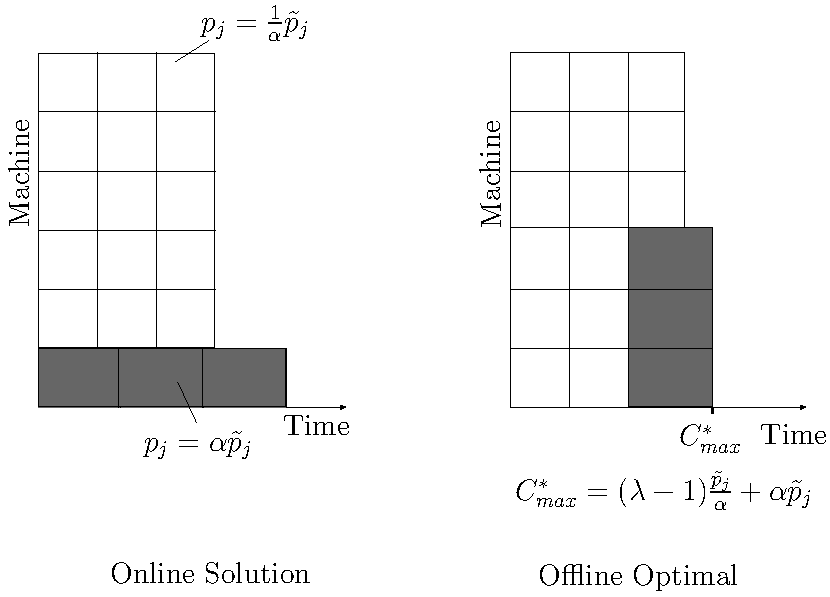
\includegraphics[width= 8 cm]{model1.pdf}
  \caption{Instance constructed by the adversary in the proof of
    theorem~\ref{th:model1-lb} with $\lambda = 3$ and $m = 6$. In the
    online solution, the adversary increased by a factor of $\alpha$
    the processing time of the task of the most loaded machine. If
    that information was available beforehand, an optimal offline
    algorithm could have distributed these longer tasks to other
    processors.}
  \label{fig:rara}
  \end{figure}
\end{proof}    
  
  
  \begin{corollary}
  When $m$ goes to $\infty$ there is no online algorithm having competitive ratio better than $\alpha^{2}$.
  \end{corollary}
  
\subsection{Algorithm}

We present the algorithm \textbf{LPT-No Choice}. In phase 1, the
algorithm distribute the data of the tasks to the processor using
their estimated processing times according to Graham's LPT
algorithm~\cite{Graham69boundson}: The tasks are sorted in non-increasing
order of their processing time and are greedily scheduled on the
processor that minimizes the sum of the $\tilde{p_i}$ of the tasks
allocated on that processor. Since there is no replication, there is
no decision to take in phase 2.

The performance of the algorithm depends mostly on how much the actual
processing times of the tasks differ from their estimation and on the
existence of a better arrangement would the actual processing time be
known. The following theorem states the theoretical guarantee of the
algorithm.

\begin{theorem}
\label{th:strat1-ub}
The \textbf{LPT-No Choice} has a competitive ratio of $ \frac{2\alpha^{2}m}{2\alpha^{2}+ m-1}$.
\end{theorem} 

\begin{proof}
  The algorithm assigns the jobs to processors based on their
  estimated processing times using LPT in Phase 1. So, the
  planned makespan considering the estimated processing times of tasks,
  $\tilde{C}_{max}$ have the following relation with the total
  estimated processing time, $\tilde{p_j}$ and estimated processing
  time of the task  $l$ that reaches $\tilde{C}_{max}$.
\begin{equation}\label{eq2}
\tilde C_{max}\leq  \frac{\sum{\tilde p_j + (m-1) \tilde p_l} }{m}
\end{equation}

The actual makespan of a schedule, $C_{max}$, obtained using the
actual processing times of all the jobs, must be smaller than $C_{max} \leq \alpha
\tilde C_{max}$ (thanks to Equation~\ref{eq1}). We
have following inequality:
\begin{equation}\label{eq3}
  C_{max}\leq \alpha \tilde C_{max}\leq \alpha \left ( \frac{\sum{\tilde p_j + (m-1) \tilde p_l} }{m} \right )
\end{equation} 

The worst case situation is when the task of the processor where the
sum of estimated processing time is $\tilde C_{max}$ sees the actual
processing time of its task being $\alpha$ times larger than their
estimate; meanwhile the processing time of the task on the rest of the
processors is $\frac{1}{\alpha}$ times their estimation. The argument
behind this statement is that greater the value of ratio
$\frac{C_{max}}{\sum{p_j}}$, the worse the algorithm approximation
ratio will be. So the total actual processing time is
given by the following equation.
 \begin{equation}\label{eq4}
 \sum {p_j} = \frac{\sum \tilde{p_j}- \tilde{C_{max}}}{\alpha} + \alpha \tilde C_{max}
 \end{equation}
 
 Also the actual optimal makespan have following constraint
 \begin{equation}\nonumber 
C_{max}^{*}\geq \frac{\sum {p_j}}{m}
\end{equation}

Substituting for  $ \sum {p_j}$, we have
 \begin{equation}\nonumber 
 m C_{max}^{*}\geq \frac{\sum \tilde{p_j}- \tilde{C_{max}}}{\alpha} + \alpha \tilde C_{max}
 \end{equation} 
\begin{equation}\nonumber 
 m C_{max}^{*}\geq \frac{\sum \tilde{p_j} - \left( \frac{\sum{\tilde{p_j} + (m-1) \tilde{p_l} }}{m} \right )} {\alpha} + {C_{max}}
\end{equation}
\begin{equation}\nonumber
 m C_{max}^{*}\geq \frac{m-1}{\alpha m} \left( \sum \tilde p_j - \tilde{p_l} \right) + {C_{max}}
 \end{equation}

 By the property of LPT, $\sum \tilde p_j-\tilde p_l \geq m (\tilde C_{max}-\tilde p_l)$, we have,
\begin{equation}\nonumber 
  m C_{max}^{*}\geq \frac{m-1}{\alpha } \left( \tilde{C_{max}} - \tilde{ p_l} \right) + {C_{max}}
 \end{equation}
 
 All instances where there is only one task per processor is always
 optimal. Therefore, we can restrict our analysis without loss of
 generality to instances with at least two jobs per processor. (Notice
 that in the original proof of Graham's LPT~\cite{Graham69boundson},
 an argument is made that all instances with two tasks per machine are
 optimal. However, the argument does not port in our case where only
 estimated processing times are known.) For at least two jobs on the
 processing that reaches having $\tilde{C}_{max}$, the (estimated)
 processing time of last job is smaller than half the estimated
 makespan, $\tilde{p_l} \leq \frac{\tilde{C}_{max}}{2}$. Substituting
 this expression in the in the above equation, we have
\begin{equation}\nonumber
 m C_{max}^{*}\geq \frac{m-1}{\alpha } \left( \tilde C_{max}-\frac{\tilde C_{max}}{2} \right ) + {C_{max}}
\end{equation}

Using equation~\ref{eq3},
\begin{equation}\nonumber
 m C_{max}^{*}\geq \frac{m-1}{2\alpha } \frac{C_{max}} {\alpha} + {C_{max}}
\end{equation}
\begin{equation}\nonumber
 m C_{max}^{*}\geq \left( \frac{m-1}{2\alpha^{2} } +1\right){C_{max}}
\end{equation}
\begin{equation}\nonumber
\frac{C_{max}}{C_{max}^{*}}\leq \frac{2\alpha^{2}m}{2\alpha^{2}+ m-1}
\end{equation}
\end{proof} 

\section{Strategy 2: replicate data everywhere}\label{sec5}

With this strategy, we put no restriction on phase 2. The tasks are
replicated everywhere i.e. $\forall j, |M_{j}|=|M|$. We introduce the
\textbf{LPT-No Restriction} which replicates the data of all the tasks
on each machine in the first phase. In the second phase we simply use
the Longest Processing Time algorithm (LPT) in an online fashion using
the estimated processing times of the task. That is to say, the tasks
are sorted in non-increasing order of their estimated processing
time. Then the task are scheduled in a greedily allocated on the first
processor that becomes available. Note that this is done in phase 2,
the processor become available with when the actual processing time of
the task scheduled onto it elapse.

\begin{lemma}\label{No Restriction}
  Let $l$ be the task that reaches $C_{max}$ in the solution
  constructed by \textbf{LPT-No Restriction}. If there are at least two
  tasks on the machine that executes $l$ in \textbf{LPT-No Restriction}, then 
  $C_{max}^* \geq {\frac{2}{\alpha^{2}}} p_l$.
\end{lemma}
\begin{proof}
  Since there are at least two tasks on the machine that executes $l$
  in \textbf{LPT-No Restriction}, there are at least $m+1$ tasks $i$
  such that $\tilde{p_j} \geq \tilde{p_l}$. Therefore in any solution
  at least one machine gets two tasks $c$ and $d$, such that $\tilde
  p_c \geq \tilde p_l$ and $\tilde p_d \geq \tilde p_l$. $C_{max}^{*}$
  must be greater than sum of the processing time of these two tasks.
   \begin{equation}\nonumber
    C_{max}^{*}\geq p_c + p_d
  \end{equation}	

  As the actual processing time of a task must be greater than  $\frac{1}{\alpha}$ times of its estimated value, we have $p_c \geq \frac{1}{\alpha}\tilde{p_c}$ and $p_d \geq \frac{1}{\alpha}\tilde{p_d}$. Using this
  \begin{equation}\nonumber 
    C_{max}^{*} \geq \frac{1}{\alpha}\tilde p_c +  \frac{1}{\alpha} \tilde p_d \geq \frac{2}{\alpha}\tilde p_l
  \end{equation}
Since, $\tilde p_l \geq \frac{1}{\alpha} p_l$, we have
  \begin{equation}\nonumber
    C_{max}^{*} \geq {\frac{2}{\alpha^{2}}} p_l 
  \end{equation}
\end{proof}

\begin{theorem}
  \label{th:strategy2}
  \textbf{LPT-No Restriction} has a competitive ratio of
  $\frac{C_{max}}{C_{max}^{*}} \leq 1 + (\frac{m-1}{m})
  \frac{\alpha^{2}}{2}$
\end{theorem} 

\begin{proof}
  The optimal makespan, $C_{max}^{*}$ must be at least equal to the
  average load on the $m$ machines. We have
  \begin{equation}\label{eq7}
    C_{max}^{*}\geq\frac{\sum p_j}{m}
  \end{equation}

  By the property of LPT (actually, it is a property of List
  Scheduling which LPT is a refinement of) the load on each machine
  $i$ is greater than the load on the machine which reach $C_{max}$
  before the last task $l$ is scheduled. So for each machine $i$,
  $C_{max} \leq \sum_{j \in E_i}^{}{p_j} + p_l$ holds true.  Summing
  for all the machines we have
  \begin{equation}\nonumber
    mC_{max} \leq  \sum {p_j} + (m-1)p_l
  \end{equation}
  \begin{equation}\label{eq8}
    C_{max} \leq  \frac{\sum {p_j}}{m} + \frac{(m-1)}{m}p_l
  \end{equation}
  
  Using~\ref{eq7} and~\ref{eq8}, we have
  \begin{equation}\nonumber
    \frac{C_{max}}{C_{max}^{*}} \leq 1 + {\frac{m-1}{m}}\left(\frac{p_l}{C_{max}^{*}}\right)
  \end{equation}
  
  Using Lemma~\ref{No Restriction}, we have 
  \begin{equation}\nonumber
    \frac{C_{max}}{C_{max}^{*}} \leq 1 + \left(\frac{m-1}{m}\right)\frac{\alpha^{2}}{2}
  \end{equation}

\end{proof}  

Graham's List Scheduling algorithm always has a competitive ratio
of $2-\frac{1}{m}$. For $\alpha^2 < 2$, the \textbf{LPT-No
  Restriction} algorithm has better approximation than List
Scheduling. For $\alpha^2 > 2$ List Scheduling has better guarantee
than the one expressed in Theorem~\ref{th:strategy2}. Since
\textbf{LPT-No Restriction} is a variant of List Scheduling,
the algorithm has a competitive ratio of $\min (1 +
\frac{m-1}{2m}\alpha^{2}, 2-\frac{1}{m})$.



\section{Strategy 3: Replication in groups}\label{sec6}


This strategy partitions the processors into $k$ groups
$G1$,$G2$...$Gk$. The size of each group is equal and have
$\frac{m}{k}$ processors within each group. For the sake of
simplicity, we assume that we will only use values of $k$ such that
$k$ divides $m$. In the first phase, the data of each task is
replicated on all the processors of one of the $k$ groups,
i.e. $\forall j, |M_j|= \frac{m}{k}$. In the second phase the tasks
are scheduled within the group they are assigned to in first phase.
Figure \ref{fig:Model 3} shows the construction of two phases in model
3.

We propose the \textbf{LS-Group} algorithm which is based on Graham's
List Scheduling algorithm. In phase 1, we use List Scheduling to
distribute the tasks to the $k$ groups of processors. In phase 2 each
task is scheduled to a particular processor within the group it was
allocated in phase 1 using the online List Scheduling algorithm.

\begin{figure*}[htp] 
\centering
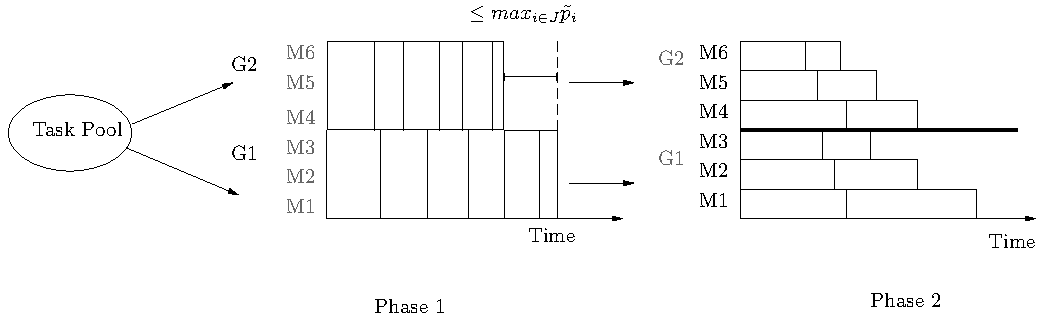
\includegraphics[width=\linewidth]{model3.pdf}
\caption{An example of replication in groups with $m = 6$, $k = 2$. In
  phase 1, the data of the tasks are assigned to one of the
  groups. Phase 2 schedules each task assigned to a machine within its
  group.}
\label{fig:Model 3}
\end{figure*}

\begin{theorem}
  \label{th:strategy3}
  With $k$ groups, the competitive ratio of
  \textbf{LS-Group } is $ \frac{k\alpha^{2}}{\alpha^{2}+k-1} (1+
  {\frac{k-1}{m}} ) + \frac{m-k}{m}$
\end{theorem}
\begin{proof} 
  We assume without loss of generality that $ C_{max}$ comes from
  group $G1$. $C_{max}^{*}$ must be greater than the average of the
  loads on the machines.
  \begin{equation}{\nonumber}
    C_{max}^{*} \geq  \frac{\sum_{i \in J}^{}{{p_{i}}}}{m}
  \end{equation}

  $\sum_{i \in T }{{p_{i}}}$ can be written as sum of load on $G1$ and
  load on rest of groups.
  \begin{equation}\label{eq11}
    C_{max}^{*} \geq  \frac{\sum_{i \in G1 }^{}{{p_{i}}}+ \sum_{l=2}^{k}\sum_{i \in Gl }^{}{{p_{i}}}}{m}
  \end{equation}

  As in phase 1 tasks are allocated to different groups using List
  Scheduling with the estimated processing times of the tasks, the
  (estimated) load difference between any two groups cannot be greater
  than the estimated value of largest task ${max_{i \in J}}{\tilde
    p_{i}}$.  So, for any group $Gl \neq G1$, We have
  \begin{equation}{\nonumber}
\forall l \in \{2, 3, \dots ,k\}, |\sum_{i \in G1 }^{}{\tilde p_{i}}- \sum_{i \in Gl }^{}{\tilde p_{i}}| \leq {max_{i \in T}}{\tilde p_{i}}
  \end{equation}  
  Adding for all values of $l$ leads to
  \begin{equation}{\nonumber}
    |(k-1)\sum_{i \in G1 }^{}{\tilde p_{i}}- \sum_{l=2}^{k}\sum_{i \in Gl }^{}{\tilde p_{i}}| \leq (k-1) {max_{i \in J}}{\tilde p_{i}}
  \end{equation}

  \textbf{Case 1:} If $(k-1)\sum_{i \in G1 }^{}{\tilde p_{i}} >
  \sum_{l=2}^{k}\sum_{i \in Gl }^{}{\tilde p_{i}}$.
  \begin{equation}{\nonumber}
    \sum_{l=2}^{k}\sum_{i \in Gl }^{}{\tilde p_{i}} \geq (k-1) \left( \sum_{i \in G1 }^{}{\tilde p_{i}}- {max_{i \in J}}{\tilde p_{i}} \right)
  \end{equation}

  As the actual processing time of the tasks can vary within a factor
  $\alpha$ and $\frac{1}{\alpha}$ of their estimated processing time,
  the following inequality holds
  \begin{equation}{\nonumber}
    \alpha\sum_{l=2}^{k}\sum_{i \in Gl }^{}{{p_{i}}} \geq (k-1) \left( \frac{1}{\alpha}\sum_{i \in G1 }^{}{{p_{i}}}- \alpha {max_{i \in J}}{{p_{i}}} \right)
  \end{equation}
  \begin{equation}\label{eq9}
    \sum_{l=2}^{k}\sum_{i \in Gl }^{}{{p_{i}}} \geq (k-1) \left(\frac{1}{\alpha^{2}}\sum_{i \in G1 }^{}{{p_{i}}}-  {max_{i \in J}}{{p_{i}}} \right)
  \end{equation}

  Phase 2 applies List Scheduling in the online mode. We assumed that
  $C_{max}$ comes from $G1$. Using the guarantees of List Scheduling
  we can write,
  \begin{equation}\label{eq10}
    C_{max} \leq \frac{\sum_{i \in G1 }^{}{{p_{i}}}}{m/k} + {\frac{m/k-1}{m/k}} p_{max}
  \end{equation}
  where $p_{max}$ is actual processing time of longest task in $G1$.

  From Equation~\ref{eq9} and~\ref{eq11}, we derive
  \begin{equation}{\nonumber}
    C_{max}^{*} \geq  \frac{\sum_{i \in G1 }^{}{{p_{i}}}+ (k-1)\left(\frac{1}{\alpha^{2}}\sum_{i \in G1 }^{}{{p_{i}}}-  {max_{i \in J}}{{p_{i}}}\right)}{m}
  \end{equation}
  \begin{equation}{\nonumber}
    \alpha^{2} (mC_{max}^{*} + (k-1){max_{i \in J}}{{p_{i}}}) \geq  (\alpha^{2} + k-1) \sum_{i \in G1 }^{}{{p_{i}}}  
  \end{equation}
  \begin{equation}\label{eq12}
    \frac{\alpha^{2}}{\alpha^{2}+k-1}\left(m C_{max}^{*}+(k-1) {max_{i \in J}}{{p_{i}}}\right) \geq \sum_{i \in G1 }^{}{{p_{i}}}  
  \end{equation}
  
  Using \ref{eq10} and \ref{eq12}, We have
  \begin{align}{\nonumber}
    C_{max} \leq \frac{k\alpha^{2}}{\alpha^{2}+k-1}\left( C_{max}^{*}+\frac{k-1}{m} {max_{i \in J}}{{p_{i}}}\right)\\
    + {\frac{m/k-1}{m/k}} p_{max} \nonumber
  \end{align}
  
  As $C_{max}^{*}\geq {{max_{i \in J}}{p_{i}}}\geq p_{max}$, we have
  \begin{align}{\nonumber}
    C_{max} \leq \frac{k\alpha^{2}}{\alpha^{2}+k-1}\left( C_{max}^{*}+ {\frac{k-1}{m}}{C_{max}^{*}}\right)\\
    + {\frac{m-k}{m}} C_{max}^{*} \nonumber
  \end{align}    
  
  So, in Case 1 the algorithm a competitive ratio of,
  \begin{equation}{\nonumber}
    \frac{C_{max}}{C_{max}^{*}} \leq \frac{k\alpha^{2}}{\alpha^{2}+k-1}\left( 1+ {\frac{k-1}{m}} \right) + {\frac{m-k}{m}} \end{equation}\\
  
  \textbf{Case 2:} If $(k-1)\sum_{i \in G1 }^{}{\tilde p_{i}} \leq \sum_{l=2}^{k}\sum_{i \in Gl }^{}{\tilde p_{i}}$. \\
  
  Since the processing times of the tasks can vary within a factor
  $\alpha$ and $\frac{1}{\alpha}$ of their estimated values, the
  expression for case 2 can be written as
  \begin{equation}{\nonumber}
    \sum_{l=2}^{k}\sum_{i \in Gl }^{}{ p_{i}} \geq \frac{1}{\alpha^2} (k-1)\sum_{i \in G1 }^{}{ p_{i}}
  \end{equation}
  
  Putting this value in equation \ref{eq11}, we have
  \begin{equation}\label{eq13}
    C_{max}^{*} \geq \frac{\alpha^2+k-1}{m\alpha^2}\sum_{i \in G1 }^{}{ p_{i}}
  \end{equation}
  Using \ref{eq10} and \ref{eq13}, and as $C_{max}^{*} \geq p_{max}$, we have
  \begin{equation}{\nonumber}
    C_{max} \leq \frac{k\alpha^2}{\alpha^2+k-1}C_{max}^{*}+\frac{m-k}{m}C_{max}^{*}
  \end{equation}
  
  So, in case 2 the algorithm has a competitive ratio of
  $\frac{k\alpha^2}{\alpha^2+k-1}+\frac{m-k}{m}$.

  Clearly, the algorithm has a worst competitive ratio in case 1.  So,
  the algorithm has a competitive approximation ratio of
  $\frac{C_{max}}{C_{max}^{*}} \leq \frac{k\alpha^{2}}{\alpha^{2}+k-1}
  \left( 1+ {\frac{k-1}{m}} \right) + {\frac{m-k}{m}}$.
\end{proof}

% \begin{corollary}
%   When there are $2$  groups, the competitive ratio is $ 1+
%   \frac{2}{1+\alpha^{2}} (\alpha^2-\frac{1}{m})$.
% \end{corollary}

\textbf{LS-Group} uses List Scheduling in both its phases. A LPT-based
algorithm may have better guarantee. But withou performing any
replication, {\em i.e.} when $k=m$, the \textbf{LS-Group} algorithm
has a competitive ratio almost equal to \textbf{LPT-No choice}'s when
the number of machines $m$ is large and the value of $\alpha$ is
within practical range. This indicates an LPT-based algorithm for
strategy 3 would likely not have a much more interesting guarantee.

\section{Summary}\label{sec7}
Table~\ref{tab:template} summarizes the results of the three
algorithms in terms of approximation ratio. Based on adversary
technique, Theorem 1.1 \todo{hardocded} states that there is no
algorithm which can give performance better than $\alpha^2$ for the
model where no replication is allowed.  LPT-No Choice is
$\frac{2\alpha^{2}m}{2\alpha^{2}+ m-1}$ approximation in this
model. For the second model having $|M_j| = |M|$ (replication
everywhere), LPT-No Restriction has a competitive ratio of $1 +
(\frac{m-1}{m})\frac{\alpha^{2}}{2}$.  The third model having $|M_j| =
m/k$, allows replication within a group of $m/k$ machines to which a
task is assigned in phase 1. For this model, LS-Group algorithm has a
competitive ratio of $\frac{k\alpha^{2}}{\alpha^{2}+k-1}\left[1+
  {\frac{k-1}{m}} \right]+ {\frac{m-k}{m}}$.



\begin{table*}[ht]
  \centering
  \begin{tabular}{|l|c|c|c|c|c|}
    \hline
    Replication & Approximation ratio  \\
    \hline
    $|M_j|=1$ & $\frac{C_{max}}{C_{max}^{*}}\leq \frac{2\alpha^{2}m}{2\alpha^{2}+ m-1}$ (Theorem~\ref{th:strat1-ub})  \\
    & No approximation better than $\frac{\alpha^{2}m }{\alpha^{2} + m-1}$ (Theorem~\ref{th:model1-lb})   \\
    
    \hline
    $|M_j|=|M|$ & $\frac{C_{max}}{C_{max}^{*}} \leq 1 + (\frac{m-1}{m})\frac{\alpha^{2}}{2}$ (Theorem~\ref{th:strategy2})  \\
    & $\frac{C_{max}}{C_{max}^{*}} \leq 2-\frac{1}{m}$ \cite{Graham66}   \\
    \hline
    
    $|M_j|= m/k $ & $\frac{C_{max}}{C_{max}^{*}} \leq \frac{k\alpha^{2}}{\alpha^{2}+k-1} \left(1+ {\frac{k-1}{m}} \right)+ {\frac{m-k}{m}}$ (Theorem~\ref{th:strategy3})  \\
%    & $\frac{C_{max}}{C_{max}^{*}} \leq  1+ \frac{2}{1+\alpha^{2}} \left(\alpha^2-\frac{1}{m}\right)$ when $k=2$ [Col. 3.1]   \\
    
    \hline
  \end{tabular}
  \caption{Summary of the guarantees of the designed algorithms.}
  \label{tab:template}
\end{table*}


To better understand the relation between these different results we
show in figure \ref{fig:Graph} how the expression of the guarantees
translate to actual values in a ratio- replication space.  We picked 3
values of $\alpha$ while keeping the number of machines fixed
$m=210$. For replication everywhere scenario the number of replication
is full and is always equal to total number of machines.  For no
replication scenario the approximation ratio is fixed for each value
of $\alpha$.  For the model where replication is allowed within the
group the approximation ratio decreases significantly with few
replications. We observe that after a significant number of
replications the ratio does not improve much further.


\begin {figure}
  \centering
  \begin{subfigure}[b]{0.5\textwidth}
    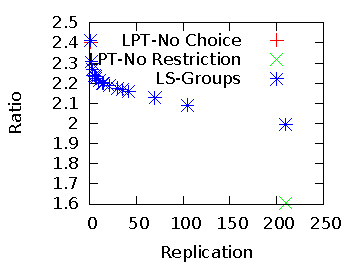
\includegraphics[width=\textwidth]{alpha_11.pdf}
    \caption{$m=210$, $\alpha=1.1$}
    \label{fig:1}
  \end {subfigure} %
  
  \begin{subfigure}[b]{0.5\textwidth}
    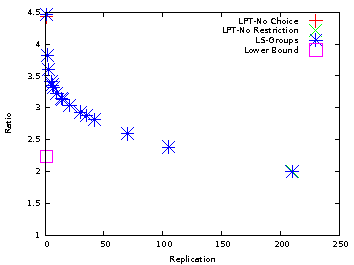
\includegraphics[width=\textwidth]{alpha_15.pdf}
    \caption{$m=210$, $\alpha=1.5$}
    \label{fig:2}
  \end {subfigure} %
  
  \begin{subfigure}[b]{0.5\textwidth}
    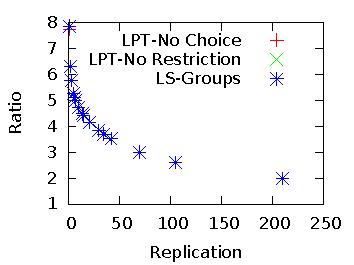
\includegraphics[width=\textwidth]{alpha_2.pdf}
    \caption{$m=210$, $\alpha=2$}
    \label{fig:3}
  \end{subfigure} %

  
  \caption{Ratio-Replication graph with m=210 and value of $\alpha$ as 1.1, 1.5 and 2}
  \label{fig:Graph}
\end{figure}

\section{Conclusion and Future Work}\label{sec8}

We study the effect on performance of parallel machine scheduling when
jobs are scheduled based on their estimated values of processing
times.  We define 3 different models which uses different replication
schemes.  We propose an approximation algorithm per model and compare
their performance. We observed that even for small amount of
replications ( i.e for small group size), the guarantee of algorithm
improves drastically. So, allowing a job to be replicated over large
number of machines (large group size) might be unnecessary.

There are some open problems which can be explored as further research
work. For models allowing more than one replica of a job, there is
scope of introducing algorithms having better lower bounds.

In this research our focus was to study the effect of replication for
minimizing makespan in scheduling under uncertainty. We did not look
in the problem through memory point of view. Replication facilitates
load balancing and allows better response time by the processors and
but it is having memory cost attached with it. So, one direction to
think about the problem would be solving bi criteria problem of
optimizing load as well as memory.
 
Algorithms that replicate task without making groups of processors
could give better guarantees as there would be no restriction on the
processors where a job can be replicated. To reduce memory cost
non-constant or selective replication can be done: replicating big
tasks only could reduce the cost of replication.


\bibliographystyle{abbrv}
\bibliography{final} 



\end{document}


